% Evaluation section for
% BigData2026__MosaicKV__Query_Forecasted_Inter_Modal_KV_Cache_Compression (1).pdf
%
% This section is derived only from canonical measurements at Git SHA
% 2d9e316398367094ab3e6f7497748e9fc43bd2ed.  It intentionally labels the
% evaluated method MosaicKV-Exact: the canonical quality-memory campaign did
% not contain verified prototype or residual-repair rows.

\section{Evaluation}
\label{sec:evaluation}

We evaluate whether query-forecasted, graph-aware selection preserves
multimodal task quality as the active KV-cache budget is reduced.  The main
experiment is a paired quality--memory study: every method receives the same
model weights, prompt, media, preprocessing, tokenizer, chat template,
generation parameters, maximum output length, precision, and attention
backend.  We use realized active KV bytes as the primary resource variable;
nominal token-retention ratios are reported only as sweep labels.  This
distinction matters because mandatory tokens and method-specific granularity
can make two nominally equal retention ratios consume different numbers of
bytes.

\subsection{Experimental Setup}
\label{sec:eval_setup}

\textbf{Models and tasks.}
We test Qwen2.5-VL-3B-Instruct, Qwen2.5-VL-7B-Instruct, and
LLaVA-1.5-7B using their pinned Hugging Face revisions.  Qwen is evaluated on
MMStar, TextVQA, DocVQA, ChartQA, and Video-MME.  LLaVA-1.5 is evaluated on the
four image tasks because this adapter does not provide the required video path.
The task metrics are MMStar average accuracy, TextVQA exact match, DocVQA
average normalized Levenshtein similarity (ANLS), ChartQA relaxed accuracy,
and the Video-MME perception score.  Scoring is delegated to the corresponding
\texttt{lmms-eval} task implementation.  We do not combine these incompatible
benchmark metrics into a macro-average.

\textbf{Methods.}
FullKV is the uncompressed reference.  RandomKV samples non-mandatory blocks
under the same byte budget, Prompt-Attention Top-K ranks blocks using only
prompt-window attention mass, and LOOK-M-reimpl is our paper-faithful local
reimplementation of LOOK-M; it is not official LOOK-M code and is evaluated
only on LLaVA-1.5.  The evaluated MosaicKV variant is
\emph{MosaicKV-Exact} (\texttt{mosaickv\_exact}): hybrid future-query
forecasting, sparse evidence-graph construction, value-aware utility, and
budgeted exact-block selection are enabled, while prototype merging and
residual repair are disabled.  No result in this section should therefore be
attributed to the prototype or repair mechanisms.  PrefixKV-reimpl,
VL-Cache-reimpl, MosaicKV-Proto, and MosaicKV-Full lacked a verified canonical
path for this campaign and are omitted instead of being represented by a
fallback or simulated result.

\textbf{Cache and generation configuration.}
Common-interface methods use 16-token blocks, with system, question, and
configured attention-sink tokens treated as mandatory.  LOOK-M-reimpl retains
its paper-faithful token granularity (block size one); its comparison is made
using actual bytes, and the granularity difference remains a design
distinction.  We sweep nominal retention ratios
\(\{1.0,0.8,0.6,0.4,0.2,0.1,0.05\}\).  MosaicKV-Exact uses the last 16 prompt
queries and four isolated greedy draft steps, four low-memory forecast
centroids, a maximum sparse-graph degree of eight, and deterministic lazy
greedy selection.  The draft rollout reuses the original prefill and is
discarded before final decoding.  Decoding is greedy with temperature zero,
\texttt{top\_p}=1, and at most 128 new tokens.

\textbf{Execution and provenance.}
All canonical rows use Hugging Face eager attention in BF16 on one NVIDIA
A100-SXM4-80GB GPU.  The software stack is Python~3.11.15, PyTorch~2.8.0,
Transformers~4.55.2, CUDA~12.8, and NVIDIA driver~595.71.05.  We use five
warmups and 20 timed repetitions for recorded timing fields.  Deterministic
methods use seed 17; RandomKV is averaged over independent selection seeds 17,
29, and 43.  Each manifest records the exact model and dataset revisions,
configuration SHA, source Git SHA, hardware, and complete backend versions.

The campaign contains 532 immutable configurations and 4,256 measured rows,
covering 14 model--task strata.  To bound execution time, each stratum uses the
same eight deterministically selected examples.  This sample size makes the
experiment a reproducible, time-bounded quality study rather than a
full-benchmark estimate; we return to this limitation in
Section~\ref{sec:eval_limits}.

\subsection{Metrics and Statistical Procedure}
\label{sec:eval_metrics}

For task metric \(s\), we report the paired score difference
\begin{equation}
    \Delta s = s_{\mathrm{method}} - s_{\mathrm{FullKV}}.
\end{equation}
The primary memory metric is the active-cache compression ratio
\begin{equation}
    r_{\mathrm{bytes}} =
    \frac{M_{\mathrm{active}}}{M_{\mathrm{FullKV}}},
\end{equation}
where both terms are computed directly from KV tensor storage.  We separately
record residual bytes; these are zero for all methods evaluated in this
section.  For diagnostic examples, token agreement is the fraction of greedy
tokens equal to the paired FullKV trajectory, and sequence agreement is one
only if the entire generated token sequence is identical.

We also measure distributional and representation fidelity.  Given FullKV
next-token distribution \(p_t\) and compressed distribution \(q_t\), logit
divergence is
\begin{equation}
    D_{\mathrm{KL}}(p_t\Vert q_t)
      = \sum_v p_t(v)\log\frac{p_t(v)}{q_t(v)}.
\end{equation}
Attention-output error is the relative layer-aggregated Frobenius error
\begin{equation}
    E_{\mathrm{attn}} =
    \sqrt{\frac{\sum_\ell\lVert A_\ell^{\mathrm{FullKV}}
    - A_\ell^{\mathrm{method}}\rVert_F^2}
    {\sum_\ell\lVert A_\ell^{\mathrm{FullKV}}\rVert_F^2}}.
\end{equation}
The diagnostic decodes clone the original prefill state and do not perform a
second prefill.

We form 95\% confidence intervals with 10,000 paired bootstrap resamples over
the eight examples in each model--task stratum.  Pareto dominance is computed
independently within each model, task, and output length.  A point is dominated
when another measured point has no lower task score and no greater resource
cost, with at least one strict inequality.  We evaluate three resource axes:
active KV bytes, end-to-end latency, and decode latency.  Because the campaign
was not fully isolated from unrelated processes on the host, memory Pareto
results are primary; latency Pareto results are diagnostic.

\subsection{Quality at Aggressive Compression}
\label{sec:eval_quality}

Table~\ref{tab:quality_r01} reports all model--task strata at nominal retention
0.1, not a selected subset.  The final column shows that mandatory-block
rounding yields 8.47--9.79\% realized active bytes for Qwen and 8.80--9.22\%
for LLaVA.  Scores are shown on a 0--100 scale; RandomKV entries are means over
three selection seeds.

\begin{table*}[t]
\centering
\caption{Task score at nominal retention 0.1.  ``Prompt'' denotes
Prompt-Attention Top-K.  LOOK-M-reimpl is a local reimplementation, not
official LOOK-M.  The active/full column is the realized MosaicKV-Exact KV-byte
ratio.  A dash denotes an unsupported combination, not a zero score.}
\label{tab:quality_r01}
\scriptsize
\resizebox{\textwidth}{!}{%
\begin{tabular}{llrrrrrr}
\hline
Model & Task (metric) & FullKV & RandomKV & Prompt & LOOK-M-reimpl & MosaicKV-Exact & Active/Full (\%) \\
\hline
Qwen2.5-VL-3B & ChartQA (relaxed) & 62.50 & 29.17 & 50.00 & -- & 62.50 & 8.47 \\
                 & DocVQA (ANLS) & 100.00 & 58.33 & 100.00 & -- & 100.00 & 9.60 \\
                 & MMStar (accuracy) & 62.50 & 62.50 & 62.50 & -- & 62.50 & 8.78 \\
                 & TextVQA (exact match) & 78.75 & 50.83 & 66.25 & -- & 78.75 & 9.47 \\
                 & Video-MME (perception) & 62.50 & 62.50 & 62.50 & -- & 62.50 & 9.79 \\
\hline
Qwen2.5-VL-7B & ChartQA (relaxed) & 75.00 & 54.17 & 62.50 & -- & 75.00 & 8.47 \\
                 & DocVQA (ANLS) & 100.00 & 65.54 & 100.00 & -- & 100.00 & 9.60 \\
                 & MMStar (accuracy) & 50.00 & 50.00 & 50.00 & -- & 50.00 & 8.78 \\
                 & TextVQA (exact match) & 78.75 & 78.75 & 66.25 & -- & 78.75 & 9.47 \\
                 & Video-MME (perception) & 62.50 & 62.50 & 62.50 & -- & 62.50 & 9.79 \\
\hline
LLaVA-1.5-7B & ChartQA (relaxed) & 0.00 & 0.00 & 0.00 & 0.00 & 0.00 & 9.22 \\
                & DocVQA (ANLS) & 41.77 & 2.08 & 31.25 & 30.83 & 6.25 & 8.80 \\
                & MMStar (accuracy) & 25.00 & 29.17 & 25.00 & 25.00 & 25.00 & 9.12 \\
                & TextVQA (exact match) & 37.50 & 0.00 & 25.00 & 12.50 & 12.50 & 9.01 \\
\hline
\end{tabular}}
\end{table*}

On both Qwen models, MosaicKV-Exact matches the measured FullKV task score in
all five strata at this budget.  The largest advantages over the equal-byte
Prompt baseline occur on ChartQA and TextVQA: MosaicKV-Exact is 12.5 percentage
points higher on each task for both model sizes.  Relative to RandomKV, the
Qwen-3B gains are 33.33 points on ChartQA, 41.67 on DocVQA, and 27.92 on
TextVQA; the corresponding Qwen-7B gains are 20.83, 34.46, and 0 points.  The
paired confidence intervals for the RandomKV losses exclude zero on Qwen-3B
ChartQA, DocVQA, and TextVQA and on Qwen-7B ChartQA and DocVQA.  In contrast,
the Prompt-baseline differences have intervals that include zero, so the
12.5-point estimates should not be described as statistically established.

These task-level results do not imply trajectory equivalence.  At retention
0.1, whole-sequence agreement is often zero and KL or attention-output error
can remain large even when the final task score matches FullKV.  The correct
interpretation is that the retained evidence was sufficient for the measured
answer metric on these examples, not that compressed decoding reproduced the
FullKV distribution.

\begin{figure*}[t]
    \centering
    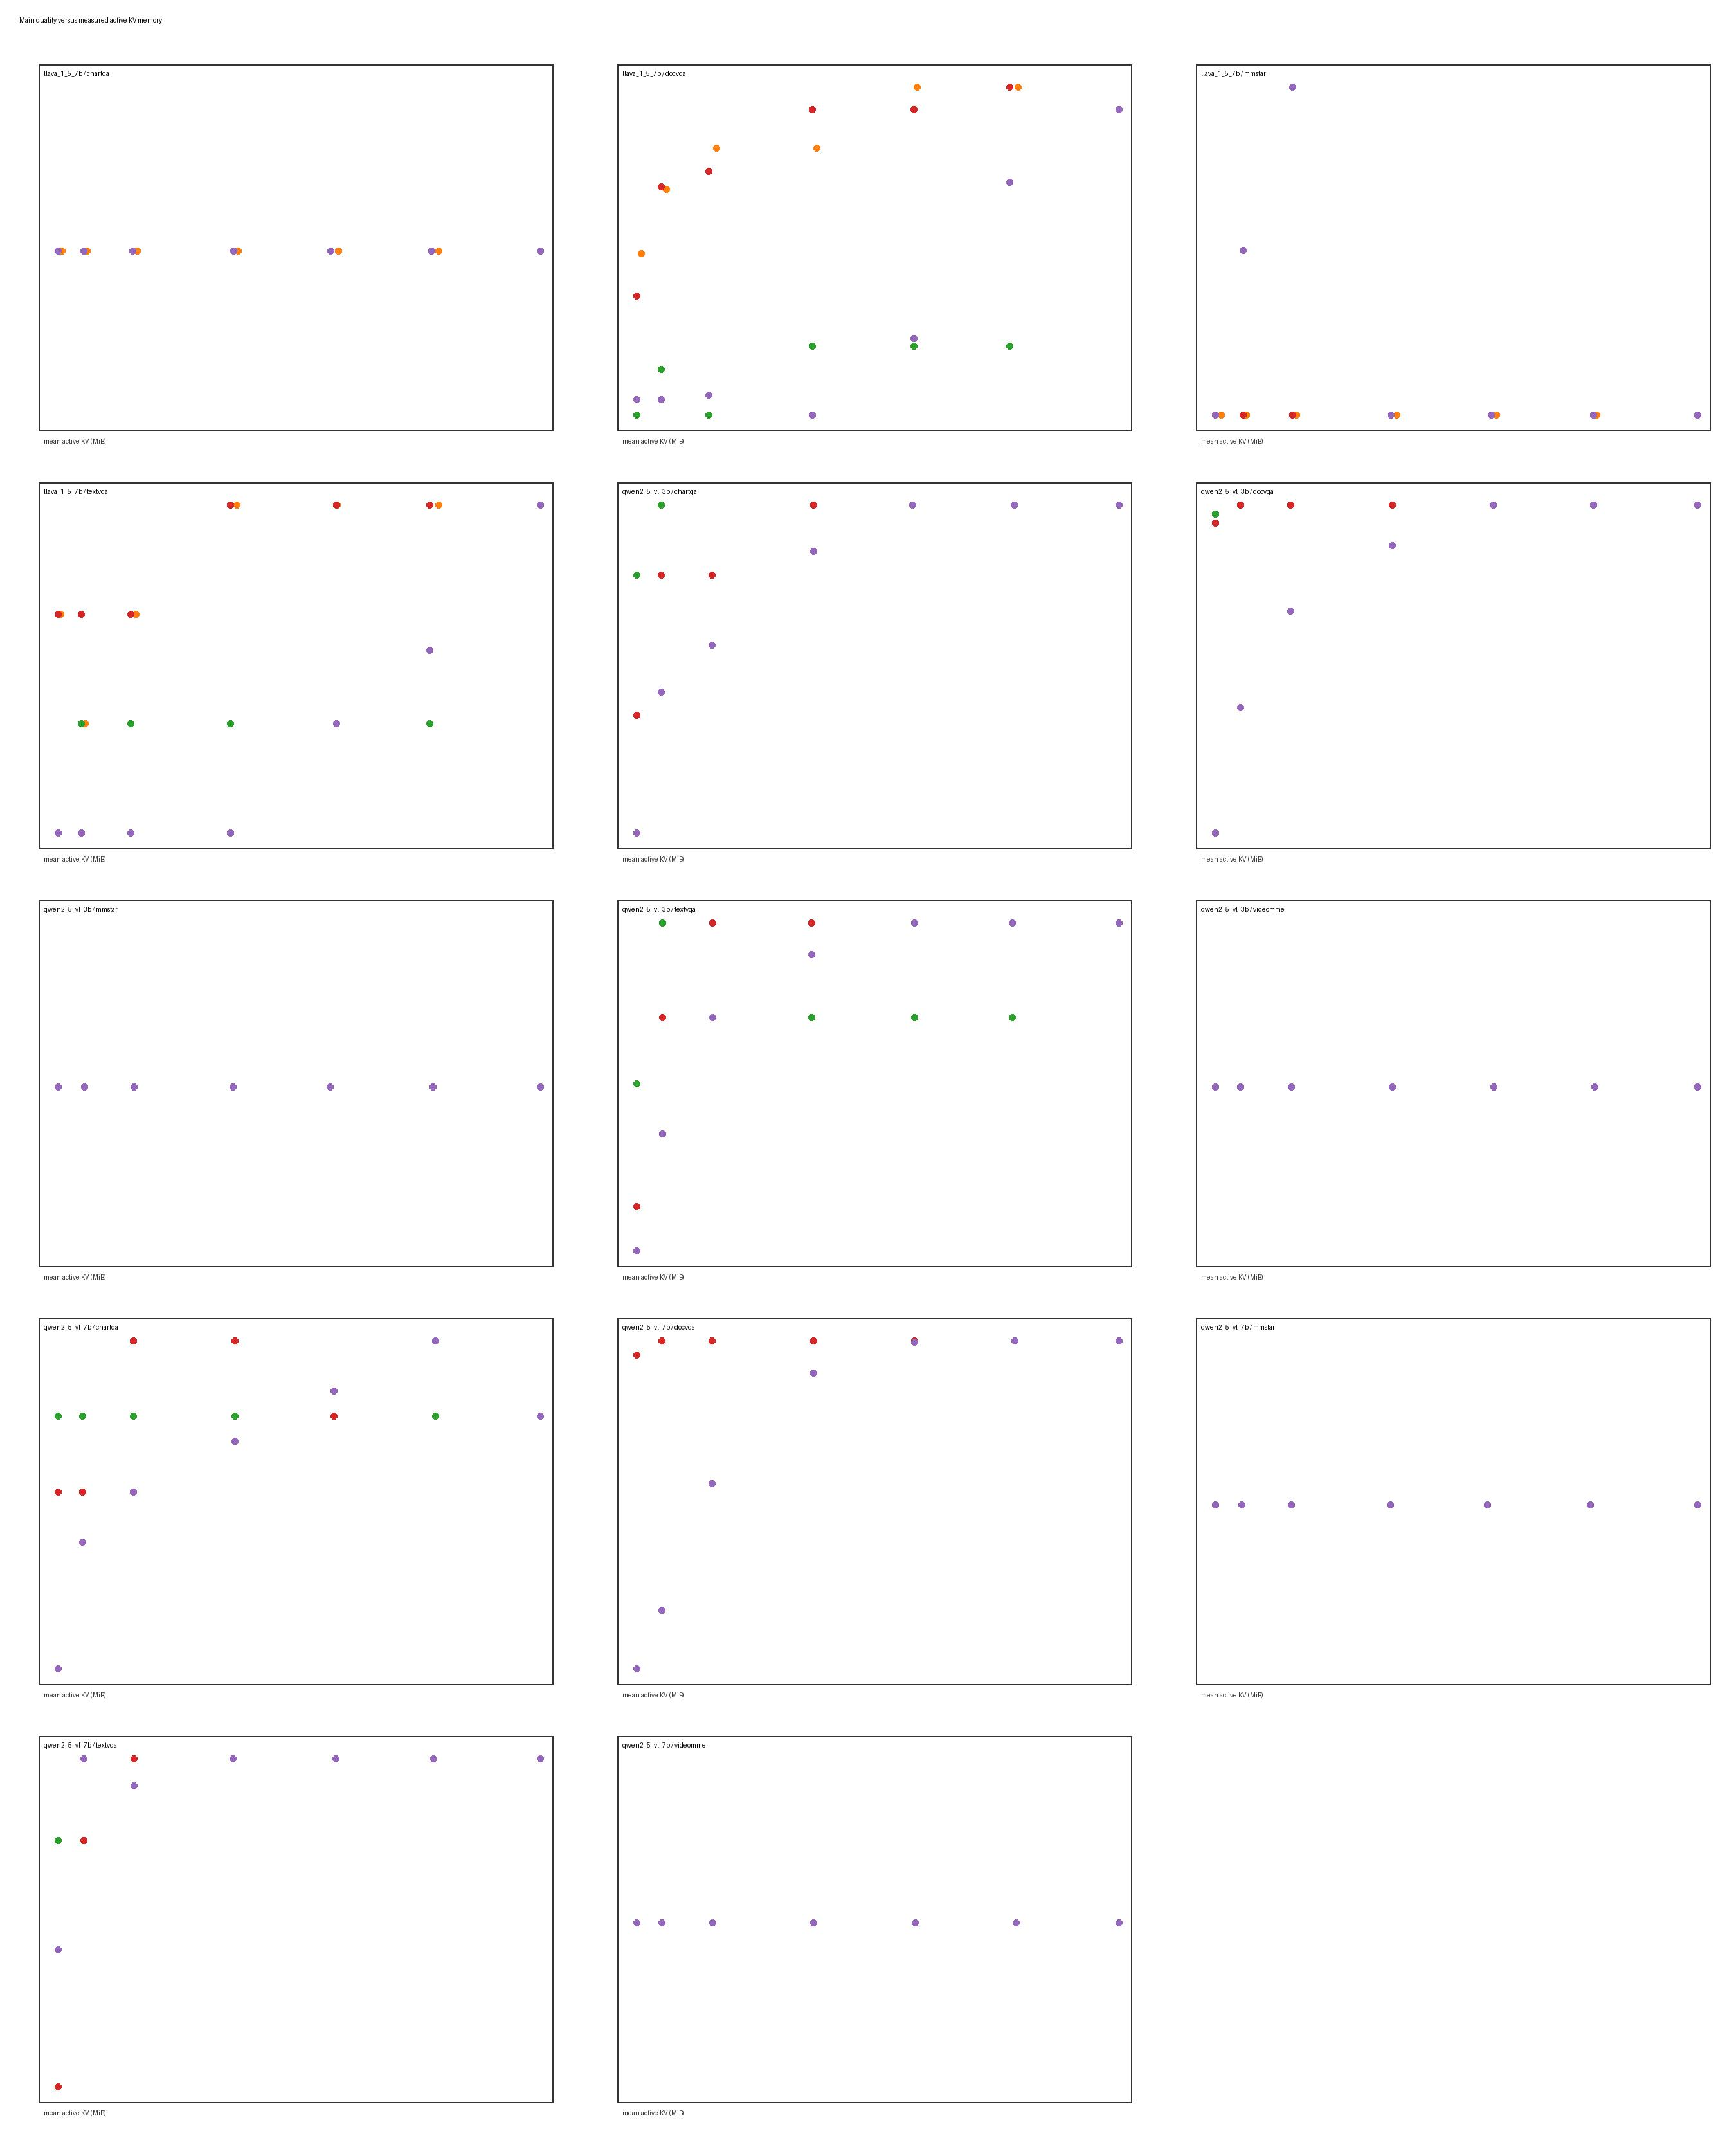
\includegraphics[width=0.96\textwidth]{mosaickv/figures/quality_memory_pareto.pdf}
    \caption{Per-model, per-task quality versus realized active KV bytes.
    Pareto status is computed within each model--task stratum; incompatible
    task metrics are never averaged.}
    \label{fig:quality_memory_pareto}
\end{figure*}

\subsection{Pareto Frontier and Mechanism-Level Interpretation}
\label{sec:eval_pareto}

Across all retention ratios, the analysis contains 336 measured
model--task--method operating points and 1,008 resource projections.
MosaicKV-Exact is Pareto-optimal in 32 of its 294 projections: 17 for quality
versus active KV bytes, 11 for quality versus decode latency, and four for
quality versus total latency.  Its active-memory frontier points are
concentrated at retention 0.05 and 0.1.  Conversely, 262 MosaicKV projections
are non-Pareto; 245 are dominated by at least one non-Mosaic baseline.  Most
notably, 94 of 98 MosaicKV total-latency projections are non-Pareto.  We
therefore find a selective memory-quality advantage rather than a general
systems-speed advantage.

The Qwen pattern is consistent with the design motivation.  RandomKV spends
the same number of bytes without estimating evidence utility and loses quality
on visually precise and document-oriented examples.  Prompt-Attention Top-K
uses a stronger signal but sees only prompt-side attention; it can miss blocks
whose relevance emerges during decoding or blocks needed to complete a
cross-modal evidence chain.  MosaicKV-Exact instead combines a prompt/draft
future-query forecast with graph coverage and value-aware utility.  At a fixed
byte budget, this objective can retain a small OCR span, chart label, or visual
region that has modest prompt attention but high forecasted contribution or
connects otherwise incomplete evidence.  This provides a mechanism-level
explanation for the ChartQA and TextVQA score estimates.

This explanation is an interpretation, not a causal conclusion from the main
experiment: the canonical campaign does not contain paper-eligible component
ablations.  A larger disjoint ablation study is required to attribute gains
separately to forecasting, graph coverage, and value-aware scoring.

\begin{figure*}[t]
    \centering
    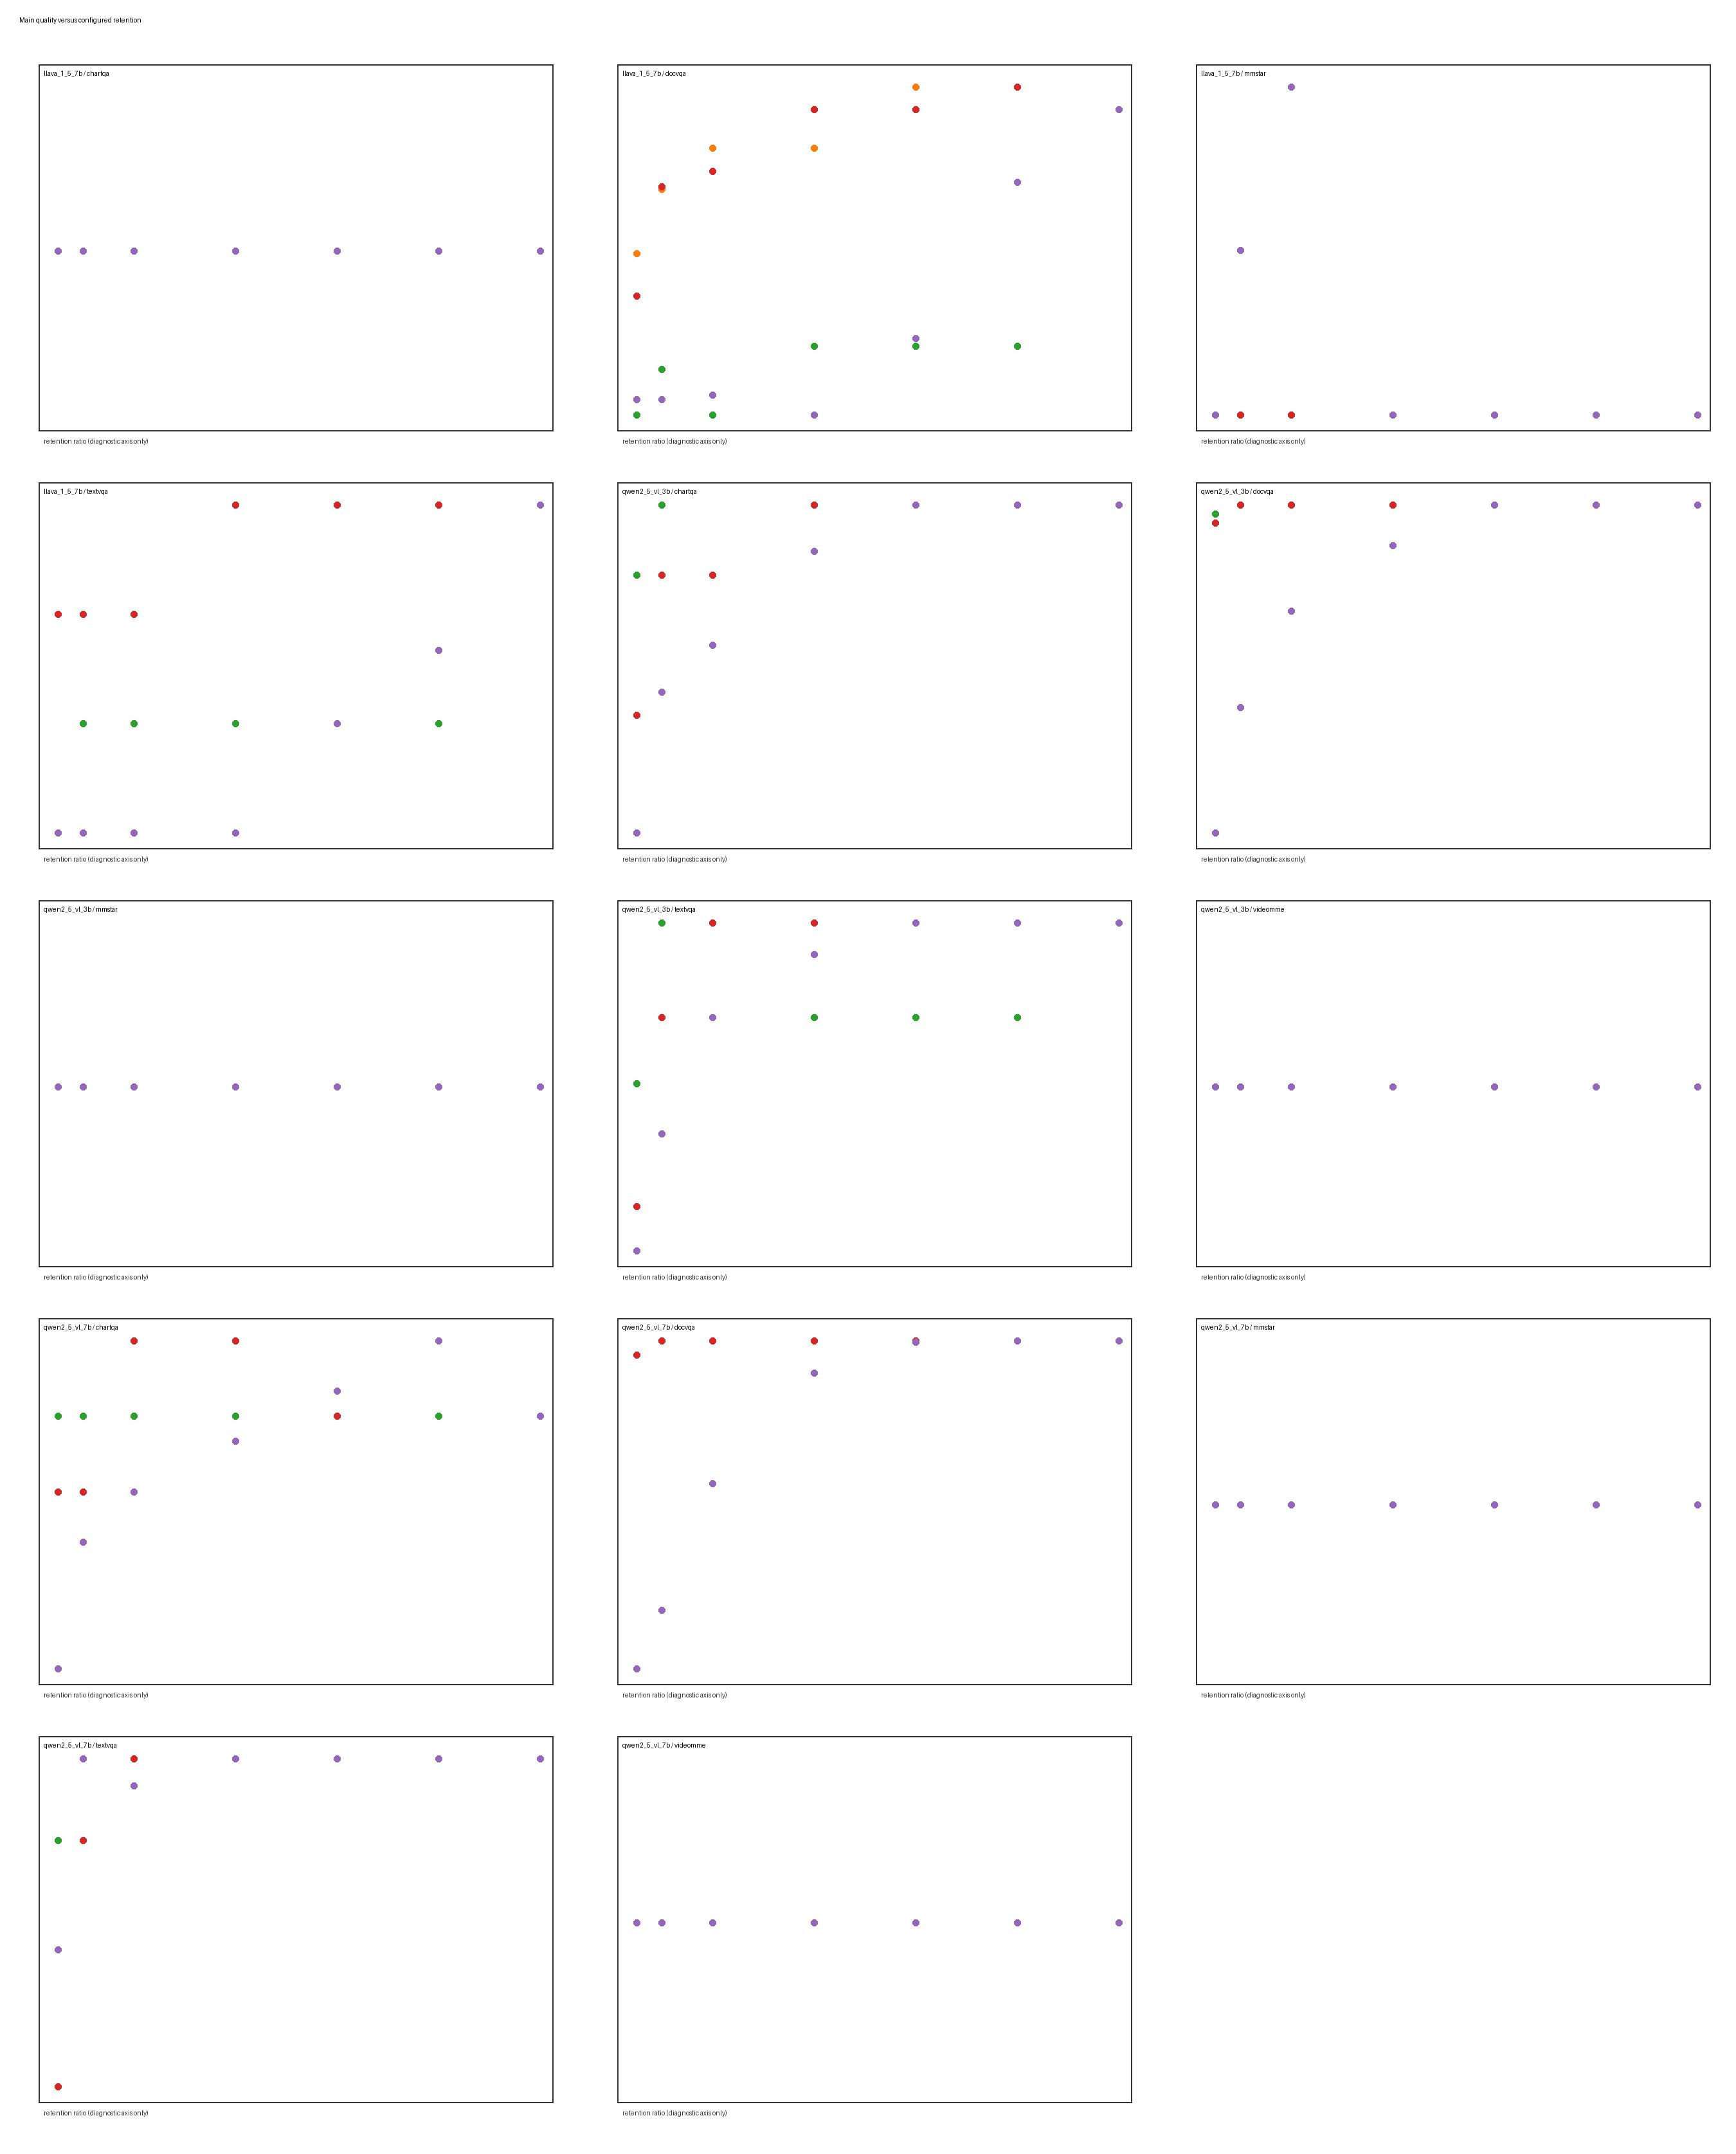
\includegraphics[width=0.96\textwidth]{mosaickv/figures/quality_retention_curves.pdf}
    \caption{Task score across nominal retention ratios.  The tables and
    Pareto analysis use realized bytes; nominal retention is used here only to
    visualize the sweep.}
    \label{fig:quality_retention}
\end{figure*}

\subsection{Correctness, Negative Results, and Limitations}
\label{sec:eval_limits}

\textbf{Full-cache equivalence.}
At retention 1.0, every compression method follows an identity path.  All 368
non-FullKV paired rows match the FullKV active-byte count and generated token
sequence exactly: token and sequence agreement are 1.0, while logit KL and
attention-output error are zero.  Three initial Video-MME attempts were
decoder-consensus outliers on corrupted videos; they were rerun with unchanged
model and experiment configurations under a larger host-memory allocation and
increased decoder EOF retries.  Superseded attempts remain archived rather
than silently removed.

\textbf{Architecture dependence.}
MosaicKV-Exact is not uniformly better.  On LLaVA-1.5 DocVQA at retention 0.1,
it scores 6.25 versus 31.25 for Prompt Top-K, 30.83 for LOOK-M-reimpl, and
41.77 for FullKV.  On LLaVA TextVQA, it scores 12.5 versus 25.0 for Prompt
Top-K and 37.5 for FullKV.  The LLaVA ChartQA subset has zero FullKV score and
cannot support a useful compression claim.  These failures indicate that the
current frozen forecast and utility configuration is not yet
architecture-general.

\textbf{Latency.}
MosaicKV-Exact pays for draft forecasting, graph construction, and lazy-greedy
selection.  Only four of 98 total-latency projections are Pareto-optimal, and
compression overhead usually exceeds the decode saving for the 128-token
outputs used here.  A faster selector or amortization over longer outputs is
needed before presenting MosaicKV as an end-to-end latency optimization.

\textbf{Statistical scope.}
Eight examples per stratum produce broad, discrete bootstrap intervals and
make individual scores sensitive to one example.  The experiment is fully
paired and provenance-complete, but it is underpowered for definitive
full-benchmark claims.  The absence of verified PrefixKV-reimpl,
VL-Cache-reimpl, prototype, and repair rows further limits the method coverage.
Accordingly, our supported conclusion is narrow: MosaicKV-Exact exposes useful
low-memory operating points on the evaluated Qwen subsets, while the present
evidence does not establish universal quality, architecture-generalization,
or end-to-end latency superiority.
